\subsection{Revsim: Reversible Logic Simulator}
  \subsubsection{Overview}

Representing reversible circuits in a way that we could both easily simulate them and process them through 
a genetic algorithm was one of the first challenges we faced. while there have been a number of reversible approaches 
to circuit synthesis using the genetic algorithm, after conducting a preliminary 
review, none of them offered the flexibility and extensibility that we were seeking. We set out to develop a 
software suite that could allow us to simulate any number of reversible circuits and let us manipulate those 
circuits at the gate level. We will provide a brief overview and description of the development of our software below.

  \subsubsection{Explanation of Simulator Design}

We first developed an initial version of our circuit simulator using a functional programming approach but once we had conducted some initial 
experimentation and testing, we decided to refactor our code using an object-oriented approach.

Figure 3 shows the basic class structure of our software. Conceptually a gate has a number of input lines, output lines, 
controls and targets. The abstract Gate class formalizes this basic representation of a gate and is subclassed to create 
the various types of gates and their implementations.

\begin{figure}[ht!]
\centering
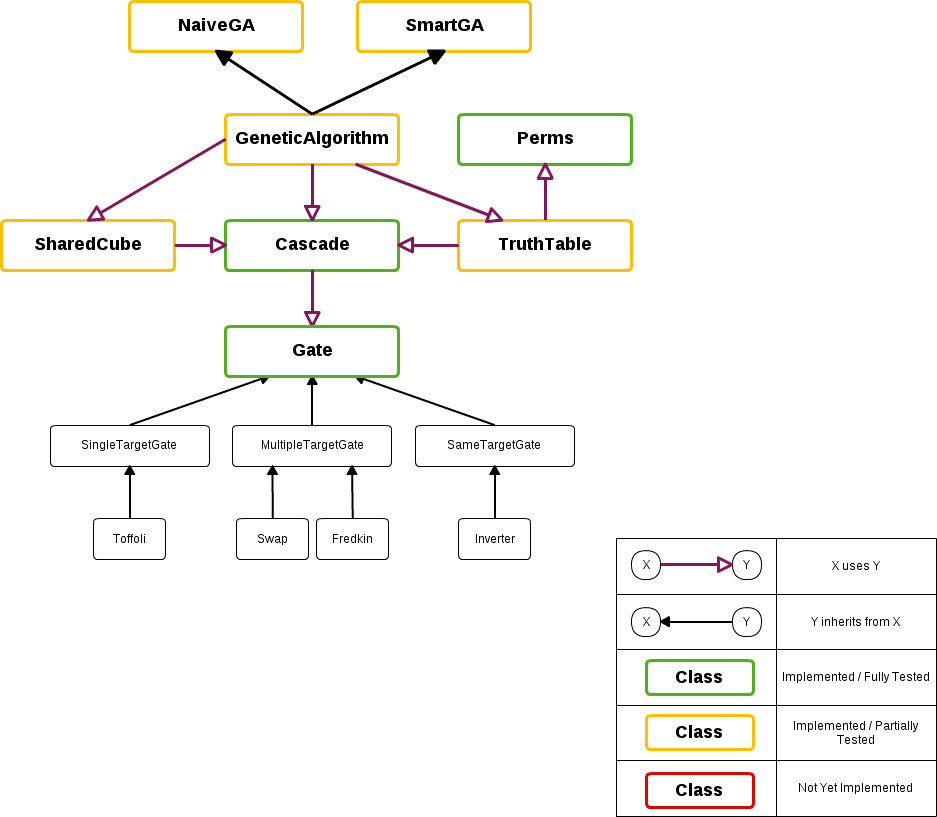
\includegraphics[width=120mm]{diagrams/architecture.png}
\caption{Class structure of Revsim}
\end{figure}

Figure 4 shows there are three main types of gates that we have represented in our simulator: Single Target 
gates, such as the the Toffoli, Multiple Target gates, like the Fredkin or Swap, and Same Target gates such as the inverter 
where the target and the control are on the same line.

\begin{figure}[ht!]
\centering
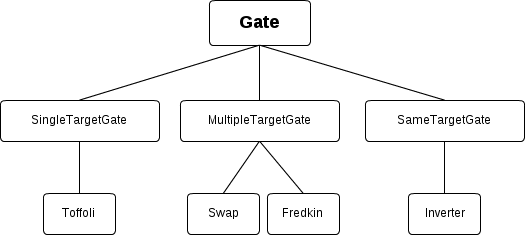
\includegraphics[width=100mm]{diagrams/gate_inheritence.png}
\caption{Gate inheritence in Revsim}
\end{figure}
The Cascade class is used to represent a reversible cascade of gates. It provides the primary functionality for modelling 
and modifying our reversible circuits, and is used other classes such as the Truth Table and Genetic Algorithm classes as 
described below.

The Truth Table class allows us to generate the truth tables of our reversible cascade and compare all or part of the truth 
table from one circuit with another. Since we have to propagate values across each gate in the cascade to generate the output 
values and need to generate all \(2^{n}\) entries in the truth table, the process of generating the truth table is linear in the 
number of gates of the circuit is exponential in the number of variables 

Our simulation software also has a number of classes that provide additional extensibility. For example there are input/output 
classes that allow us to directly read from and write to files in the \url{www.revlib.org}'s .real file format. Our initial genetic algorithm implementation 
required us to manually enter each goal cascade that we wanted to test against, but using these helper classes we were able to 
implement the ability to parse any .real file and use its target output function in the fitness calculations for our genetic 
algorithm. We also developed an experimental Shared Cube class that allows us to generate and use the shared cube 
representation that we were initially going to use to represent individuals in our genetic algorithm so that we could apply a 
number of the rule based transformations from \cite{Nayeem2011} but after implementing it, we decided 
on using the representation described below. 

  \subsubsection{Description of Our Genetic Algorithm}

\paragraph{Representation.} 

We initially explored using a shared cube representation for the individuals in used in our algorithm however while we initially 
thought that the transformational rules  in \cite{Thornton2007} would be useful in implementing mutation, we found it difficult to implement 
in the context of our genetic algorithm and we were not able to discover an appropriate method of implementing crossover using the shared 
cube representation. Instead. we settled on using the cascade representation from our Cascade class which stores the list of gates used 
in the circuit for the individuals in our populations.

Our algorithm initially reads in a circuit that specifies the desired output behaviour and then creates the initial population as copies 
of the initial circuit that have been mutated from the initial circuit up to a maximum number of mutations specified in the initial 
conditions. Once the initial population is generated, the cycle of fitness evaluations, selection, mutation and crossover repeats until 
one of two terminal conditions are reached, either a fitness of 1.0 or a maximum number of generations.

\paragraph{Fitness and Selection.} 

Our fitness metric measured how closely the truth table of the current individual matched the truth table of the of 
the desired output behaviour. It basically performs an exhaustive comparison and so the number of comparisons needed are approximately
 exponential in the number of variables (linewidth) of the circuit.  


\paragraph{Crossover.}

Our implementation of crossover selects the best two individuals as parents and creates two child individuals. The first child has the 
first half of the gates from parent 1 and the second half from parent 2 while the second child has the first half of the gates from 
parent 2 and the second half from parent 1. The children are then added to the population for the next iteration of the algorithm. 

\paragraph{Mutation.}

The mutation function randomly selects a certain number of gates and will either replace or remove them from the cascade of the 
individuals it is being applied to.

\paragraph{Parameter Variations.}

Our initial parameters


\subsubsection{Parallelization}

We found that with larger circuits processing time became significantly longer so we looked at a few ways to parallelize our simulations 
in order to gather a larger dataset of results in a shorter period of time.

\paragraph{Grid Computing.}

We first spent some time adapting our software so that we could run it across the university of Lethbridge's HTcondor computing grid. 
Because we needed to test a number of circuits across a set of variable initial parameters one of the key challenges we faced was 
automating the task of creating the HTcondor job submissions. We were able to script a solution that allows us to automatically take 
a batch of any number reversible circuits in .real format and output a set of submission-ready executables that we could run across 
the HTcondor grid. This provided a significant increase in the speed we were able to generate tests and obtain results.

\paragraph{Parallelization of large circuits.}

Even using condor we still faced the problem that that the processing time for runs of our genetic algorithm with large circuits was 
significantly longer. In order to mitigate this we began experimenting with spitting the processing of each individual circuit into 
multiple processes that we can run concurrently on each of the processors of the machine running the job. Preliminary tests have been 
promising.   \emph{  DOUBLE CHECK THIS STATEMENT!!! is is really promising??}